% MTH321 Project 2, Direction 2 (elliptic BVP, mixed boundary data) -- Team F talk.
% Build: latexmk -pdf main.tex.  Figures: copied from ../report/figures (drawn by ../code/d2_extra.py, TeX Gyre Pagella).
% Numbers: ../report/tables/*.tex, ../results/d2_extra_log.txt, ../report/main.tex. Nothing else.
\documentclass[aspectratio=169,8pt,t]{beamer}
% =====================================================================
% polish_preamble.tex -- Team F talk preamble: palette, hairlines, theorem style, sizes
% (body 10pt, frame titles 12pt, tables 9pt, captions 8pt), old-style figures in text,
% lining figures in math, quiet section navigation in the footer.
% =====================================================================
\usefonttheme{serif}
\usefonttheme{professionalfonts}
\usepackage{amsmath}
\usepackage{fontspec}
\usepackage[math-style=TeX,bold-style=TeX]{unicode-math}
\setmainfont{TeX Gyre Pagella}[Numbers={Lining,Proportional}]   % Palatino text, lining figures
\setsansfont{TeX Gyre Pagella}[Numbers={Lining,Proportional}]   % no stray sans anywhere
\setmonofont{TeX Gyre Pagella}[Numbers=Lining]
\setmathfont{texgyrepagella-math.otf}                              % matching Palatino math
\usepackage{array}
\linespread{1.18}

% ---------- palette --------------------------------------------------------
\definecolor{ink}{HTML}{1F2933}
\definecolor{accent}{HTML}{23426B}
\definecolor{muted}{HTML}{4B5563}   % secondary text, lighter than ink
\definecolor{hairline}{HTML}{C9CDD2}
\definecolor{note}{HTML}{374151}     % page-bottom notes and captions (darker than muted)
\definecolor{navcur}{HTML}{C2642B}   % current section in the footer nav (muted burnt orange)
\definecolor{hlY}{HTML}{FFEB99}
\definecolor{hlG}{HTML}{CDEBC5}
\definecolor{hlR}{HTML}{F9D3C4}
\definecolor{boxred}{HTML}{B03A2E}
\definecolor{lineblue}{HTML}{2F5D8C}
\setbeamercolor{normal text}{fg=ink,bg=white}
\setbeamercolor{background canvas}{bg=white}
\setbeamercolor{structure}{fg=accent}
\setbeamercolor{alerted text}{fg=boxred}
\setbeamercolor{frametitle}{fg=accent,bg=}
\setbeamercolor{footline}{fg=accent}   % footer in the structure navy
\setbeamercolor{itemize item}{fg=muted}
\setbeamercolor{enumerate item}{fg=muted}

% ---------- sizes -------------------------------------------------------------
\setbeamerfont{frametitle}{size=\fontsize{12}{14.5}\selectfont}
\setbeamerfont{footline}{size=\fontsize{7.5}{9}\selectfont}

% ---------- layout --------------------------------------------------------------
\setbeamersize{text margin left=8mm,text margin right=8mm}
\setbeamertemplate{navigation symbols}{}
\setbeamertemplate{headline}{}
\setbeamertemplate{frametitle}{%
  \vskip 1.6mm% fixed-height title box: rule at the same y on every page
  \hbox to\textwidth{\usebeamerfont{frametitle}\usebeamercolor[fg]{frametitle}\rule{0pt}{4.2mm}\smash{\insertframetitle}\hfil}%
  \nointerlineskip\vskip 3.45mm\hbox{\color{hairline}\rule{\textwidth}{0.4pt}}\vskip -2.6mm}
% quiet agenda in the footer: the current part in accent, the others in muted small caps
\newcommand{\navitem}[2]{\ifnum\value{section}=#1{\color{navcur}\textsc{#2}}\else\textsc{#2}\fi}   % current part in burnt orange
\newcommand{\navsep}{\hspace{0.9em}}
\setbeamertemplate{footline}{%
  \usebeamerfont{footline}\usebeamercolor[fg]{footline}%
  \hbox to \paperwidth{\hskip 8mm\rlap{\textsc{Mixed boundary data}\ \textperiodcentered\ \textsc{Team F}}\hfill
    \navitem{1}{model}\navsep\navitem{2}{analysis}\navsep\navitem{3}{experiments}\navsep
    \navitem{4}{close}\hfill
    \llap{\insertframenumber\,/\,\inserttotalframenumber}\hskip 8mm}\vskip 3.6mm}
\addtobeamertemplate{frame begin}{}{\raggedright\hyphenpenalty=10000\exhyphenpenalty=10000}
\hyphenpenalty=10000 \exhyphenpenalty=10000
\setbeamertemplate{itemize item}{\raisebox{0.12ex}{\textendash}}
\setbeamertemplate{enumerate item}{\insertenumlabel.}
\setlength{\leftmargini}{1.4em}

% ---------- theorem-like: small-caps label, no coloured blocks ------------------
\setbeamertemplate{theorems}[normal font]
\setbeamertemplate{theorem begin}{\par\addvspace{\blockskip}\noindent
  {\upshape\scshape\color{accent}\inserttheoremname}%
  \ifx\inserttheoremaddition\empty\else\ {\color{muted}(\inserttheoremaddition)}\fi.\ \itshape}
\setbeamertemplate{theorem end}{\par\addvspace{\blockskip}}
\newtheorem*{proposition*}{Proposition}
\newtheorem*{remark*}{Remark}

% ---------- no emphasis marks: no boxes, underlines or highlights -------------------
\newcommand{\dfn}[1]{{\color{accent}#1}}
\newcommand{\notesize}{\fontsize{8.5}{10.6}\selectfont}         % notes/captions 8.5pt
\newcommand{\notesizesmall}{\fontsize{7.5}{9.4}\selectfont}    % AI-use block 7.5pt
\newcommand{\aside}[1]{{\color{note}\notesize\upshape #1}}
\newcommand{\figcap}[1]{{\color{note}\notesize\upshape #1\par}}   % \par inside: footnotesize leading

% ---------- tables and display spacing ---------------------------------------------
\usepackage{booktabs}
\setlength{\aboverulesep}{0.3ex}\setlength{\belowrulesep}{0.45ex}
\setlength{\heavyrulewidth}{0.6pt}\setlength{\lightrulewidth}{0.35pt}\setlength{\cmidrulewidth}{0.35pt}
\renewcommand{\arraystretch}{1.1}
\newcommand{\tabfont}{\small\addfontfeatures{Numbers={Lining,Monospaced}}}   % 9pt, lining figures so table columns align
\newcommand{\stack}[1]{\begin{tabular}[t]{@{}l@{}}#1\end{tabular}}   % manual line break inside a cell
\makeatletter
\g@addto@macro\normalsize{\setlength\abovedisplayskip{5pt}\setlength\belowdisplayskip{5pt}%
  \setlength\abovedisplayshortskip{4pt}\setlength\belowdisplayshortskip{4pt}}
\makeatother

% ---------- layout rhythm ---------------------------------------------------
% every frame body starts \bodytop below the title rule; footnote-style asides sit \asidegap above the footer
\newlength{\bodyskip}\setlength{\bodyskip}{0.6mm}
\newlength{\blockskip}\setlength{\blockskip}{3.0mm}% the one fixed gap between body blocks
\newcommand{\bodytop}{\vspace*{\bodyskip}\vspace*{1.6mm}\vspace{0pt plus 0.3fill}}
\newcommand{\tabletop}{\vspace*{\bodyskip}\vspace*{2.5mm}}   % table top rule level with the cap height of text pages
\newcommand{\closing}[1]{\par\addvspace{\blockskip}{\color{note}\notesize\upshape #1\par}\vspace{0pt plus 1fill}}
\newcommand{\figend}[1]{\par\vspace{\blockskip}{\color{note}\notesize\upshape #1\par}\vspace{0pt plus 1fill}}   % figure frames: tighter bottom gap
\newcommand{\blockgap}{\par\addvspace{\blockskip}}     % between body blocks (table -> text, list -> text)
\newcommand{\colgap}{\par\vspace{\blockskip}}       % between paragraphs inside the text column of figure frames
\newcommand{\lead}[1]{{\upshape\scshape\color{accent}#1}}   % small-caps run-in label (Goal, Remark)

% ---------- stroke weight: text drawn fill+stroke with a hairline stroke in the text colour ----
% Palatino stays Palatino; glyphs gain ~0.1pt per side, so the deck reads better when projected.
% Text remains real text (selectable, searchable); colours unchanged (xcolor sets fill and stroke).
\usepackage{pdfrender}
\newcommand{\strokeweight}{0.15pt}
\AtBeginDocument{\pdfrender{TextRenderingMode=FillStroke,LineWidth=\strokeweight,LineJoinStyle=1}}
% ---------- Project 2 additions ----------
\definecolor{todo}{HTML}{B03A2E}
\newcommand{\TODO}[1]{{\color{todo}[TODO: #1]}}

\setlength{\parskip}{0pt}
\AtBeginDocument{\renewcommand{\setminus}{\mathbin{\backslash}}}

%\renewcommand{\ttdefault}{pcr}
\setbeamerfont{frametitle}{size=\fontsize{10.5}{12.5}\selectfont}
\graphicspath{{figures/}}
\newcommand{\GD}{\Gamma_D}\newcommand{\GB}{\Gamma_B}\newcommand{\dd}{\,\mathrm{d}}
\title{Mixed boundary data for the Poisson equation}
\hypersetup{pdftitle={Mixed boundary data for the Poisson equation: first-order versus ghost-point closures},
  pdfauthor={Team F}, pdfsubject={MTH321 Project 2, Direction 2}}
% text-style fraction gaps with display-size parts (slide 5)
\newcommand*{\tfracD}[2]{\genfrac{}{}{}{1}{\displaystyle #1}{\displaystyle #2}}
\begin{document}
\section{Model}
% ============================================================ 1 title
{\setbeamertemplate{background}{\vbox to \paperheight{\vfill
  \usebeamerfont{footline}\usebeamercolor[fg]{footline}%
  \hbox to \paperwidth{\hfill\llap{\insertframenumber\,/\,\inserttotalframenumber}\hskip 8mm}\vskip 3.6mm}}
% XJTLU crest (shield only), vector PDF: figures/xjtlu_crest.pdf (+ .svg).
%   Source: official XJTLU logo SVG on xjtlu.edu.cn,
%     https://www.xjtlu.edu.cn/wp-content/uploads/2024/01/cn-footer-logo-light.svg
%   as used on https://www.xjtlu.edu.cn/en/about/overview/xjtlu-identity .
%   Shield paths extracted unchanged; the reversed-out (light) colours were swapped
%   to the positive navy shield (#010544) with white charges, as in the official
%   logo on that page. Converted SVG -> PDF with rsvg-convert (vector, no raster).
%   Licence: the XJTLU logo is a registered trademark of Xi'an Jiaotong-Liverpool
%   University (see https://www.xjtlu.edu.cn/en/about/brand-resources); used here
%   only to identify the institution on a non-commercial student coursework talk.
% Placement: height 14mm, right edge on the 8mm right margin, top aligned with the
% small-cap height of the cover's top text line.
\newlength{\crestcap}
\begin{frame}[plain]
\vspace*{0pt plus 1filll}
\hspace*{6mm}\begin{minipage}{0.86\textwidth}\raggedright
{\color{note}\notesize\settoheight{\crestcap}{\textsc{mth}}%
\leavevmode\rlap{\hspace*{\dimexpr\paperwidth-22mm\relax}\llap{\raisebox{\dimexpr\crestcap-14mm\relax}[0pt][0pt]{
\includegraphics[height=14mm]{xjtlu_crest}}}}%
\textsc{mth321}\ \textperiodcentered\ \textsc{project 2}\ \textperiodcentered\ \textsc{direction 2: elliptic bvp, mixed boundary data}}\par\vspace{5mm}
{\color{accent}\fontsize{13}{16.5}\selectfont Mixed boundary data for the Poisson equation\par}\vspace{1.6mm}
{\itshape First-order versus ghost-point closures of a five-point scheme\par}\vspace{3.5mm}
{\color{hairline}\rule{0.42\textwidth}{0.4pt}}\par\vspace{3.2mm}
{\textsc{Team F}}\par\vspace{1.6mm}
{\footnotesize
\begin{minipage}[t]{0.46\textwidth}\raggedright
Kunze Li, 2363973 --- Project Manager\\
Yawen Wu, 2360749 --- Mathematical Theory\\
Che Li, 2362072 --- Algorithm Implementation
\end{minipage}\hfill
\begin{minipage}[t]{0.50\textwidth}\raggedright
Zekun Wang, 2363718 --- Visualization \& Report\\
Yixuan Liu, 2361140 --- Testing \& Validation\\
Ruitong Huang, 2360294 --- Video \& presentation
\end{minipage}\par}\vspace{3.5mm}
{\color{accent}\footnotesize Xi'an Jiaotong-Liverpool University}\par
\end{minipage}
\vspace*{0pt plus 1.25filll}
\end{frame}}

% ============================================================ 2 problem
\begin{frame}{The problem: Dirichlet data on three edges, a flux law on the fourth}
\bodytop
On $\Omega=(0,1)^2$ let $\GB=\{1\}\times(0,1)$ be the open right edge and $\GD=\partial\Omega\setminus\GB$ (owns all four corners). Seek $u$ with
\[
-\Delta u=f\ \text{in }\Omega,\qquad u=g\ \text{on }\GD,\qquad \partial_n u+\beta u=r\ \text{on }\GB,\qquad \partial_n u=u_x .
\]
Neumann: $\beta=0$, $r=q$. Robin: $\beta=2$.
\blockgap
\lead{Manufactured solution} (Problem Pack): $u^*=e^{x+y}$, $f=-2e^{x+y}$, $g=u^*|_{\GD}$, $q=e^{1+y}$, $r=(1+\beta)e^{1+y}$. Sign check $q>0$: outward normal, $u^*$ increases towards $\GB$.
\blockgap
\lead{Question} (Direction 2). How does the flux-edge closure decide the global order of a five-point scheme, and what does it do to the linear system?
\closing{Steady heat conduction with convective Robin exchange (Bergman--Incropera et al., 2011); pressure-Poisson with Neumann wall data (Gresho--Sani, 1987).}
\end{frame}

% ============================================================ 3 well-posedness
\begin{frame}{Well-posedness: Lax--Milgram, provided $\beta\ge 0$}
\bodytop
With $V=\{v\in H^1(\Omega):v|_{\GD}=0\}$ and a lifting $g_\ast$ of $g$: find $u\in g_\ast+V$ with
\[
a(u,v)=\int_\Omega\nabla u\cdot\nabla v\dd x+\beta\int_{\GB}uv\dd s=\int_\Omega fv\dd x+\int_{\GB}rv\dd s=\ell(v)\qquad\forall v\in V.
\]
\begin{proposition*}
If $f\in L^2(\Omega)$, $r\in L^2(\GB)$, $g=\operatorname{tr}g_\ast$ for $g_\ast\in H^1(\Omega)$ and $\beta\ge0$ constant, the weak problem has a unique solution depending continuously on $(f,r,g_\ast)$.
\end{proposition*}
\begin{itemize}\setlength{\itemsep}{\blockskip}
\item Boundedness: Cauchy--Schwarz and the trace inequality $\|v\|_{L^2(\GB)}\le C_T\|v\|_{H^1}$.
\item Coercivity: $\GD$ has positive length $\Rightarrow$ Friedrichs on $V$ with $C_P=1/\sqrt2$; for $\beta\ge0$, $a(v,v)\ge\|\nabla v\|^2\ge(1+C_P^2)^{-1}\|v\|^2_{H^1}$.
\item Sign: coercivity uses $\beta\int_{\GB}v^2\ge0$, so only $\beta\ge0$ is claimed. $\GD$ has positive measure $\Rightarrow$ no compatibility condition.
\end{itemize}
\closing{Orders below assume $u\in C^4$ up to $\GB$; mixed problems may lose regularity at $(1,0)$, $(1,1)$ (Grisvard). Not claimed for nonsmooth data.}
\end{frame}

\section{Analysis}
% ============================================================ 4 discretisation
\begin{frame}{Discretisation: one stencil, two closures of the flux edge}
\bodytop
$h=1/N$; unknowns $U_{i,j}$, $1\le i\le N$, $1\le j\le N-1$ ($M=N(N-1)$; Dirichlet values to the RHS). Interior, $1\le i\le N-1$:
\[
\bigl(4U_{i,j}-U_{i-1,j}-U_{i+1,j}-U_{i,j-1}-U_{i,j+1}\bigr)/h^2=f_{i,j}.
\]
\lead{Closure 1, first-order row.} Replace the PDE row at $(N,j)$ by a backward difference of the BC:
\[
\Bigl(\tfrac1h+\beta\Bigr)U_{N,j}-\tfrac1h U_{N-1,j}=r_j .
\]
\lead{Closure 2, ghost point.} Impose $(U_{N+1,j}-U_{N-1,j})/(2h)+\beta U_{N,j}=r_j$ and eliminate $U_{N+1,j}$:
\[
\Bigl(\tfrac4{h^2}+\tfrac{2\beta}h\Bigr)U_{N,j}-\tfrac2{h^2}U_{N-1,j}-\tfrac1{h^2}\bigl(U_{N,j-1}+U_{N,j+1}\bigr)=f_{N,j}+\tfrac2h r_j .
\]
Closure 1 enforces only the BC (scale $h^{-1}$); closure 2 keeps the PDE with the BC built in (scale $h^{-2}$).
\closing{Residuals compared only in the row-scaled form $\rho=\max_k|(F-AU)_k|/(|A||U|+|F|)_k$, invariant under these scalings.}
\end{frame}

% ============================================================ 5 truncation
\begin{frame}{Truncation error: both boundary rows are only $O(h)$}
\bodytop
\begin{columns}[T,onlytextwidth]
\column{0.50\textwidth}
With $\tau=A\,u^*|_{\mathrm{grid}}-F$ and Taylor at $(1,y_j)$:
{\setlength{\abovedisplayskip}{0.35em}%
\setlength{\belowdisplayskip}{0.45em}%
\setlength{\abovedisplayshortskip}{0.2em}%
\setlength{\belowdisplayshortskip}{0.3em}%
\[
\begin{aligned}
\tau_{i,j}
  &= -\tfracD{h^{2}}{12}\,(u_{xxxx}+u_{yyyy})+o(h^{2})
     \quad(u\in C^{4}),\\
\tau^{(1)}_{N,j}
  &= -\tfracD{h}{2}\,u_{xx}(1,y_{j})+O(h^{2}),\\
\tau^{(2)}_{N,j}
  &= \phantom{-}\tfracD{h}{3}\,u_{xxx}(1,y_{j})+O(h^{2}).
\end{aligned}
\]}

For $u^*$: $\max|\tau_B|/h\to e^2/2$ (first), $e^2/3$ (ghost); $\max|\tau_I|/h^2\to e^2/6$. Local order alone does not explain different global orders.
\colgap
{\tabfont\begin{tabular}{@{}lccc@{}}\toprule
Robin, $N=256$ & $\max|\tau_B|/h$ & predicted & $\max|\tau_I|/h^2$\\\midrule
first-order & 3.6753 & 3.6945 & 1.2219\\
ghost-point & 2.4486 & 2.4630 & 1.2219\\\bottomrule
\end{tabular}}\blockgap
{\color{note}\notesize Substituting $u^*$ into the assembled rows.\par}
\column{0.04\textwidth}
\column{0.46\textwidth}
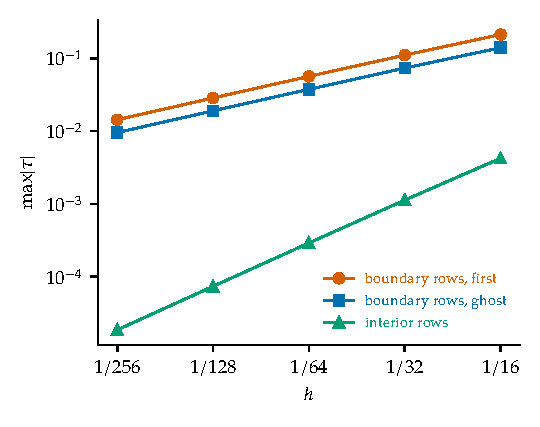
\includegraphics[width=0.92\textwidth]{truncation.pdf}\par\vspace{1mm}
\figcap{Robin, $\max|\tau|$ vs $h$: both boundary rows $\sim h$, interior $\sim h^2$.}
\end{columns}
\end{frame}

% ============================================================ 6 matrix SPD
\begin{frame}{Matrix structure: $DA$ symmetric positive definite}
\bodytop\vspace{-\blockskip}
\begin{proposition*}
Let $D=\operatorname{diag}(d_k)$ with $d_k=1$ on five-point rows and, on right-edge rows, $d_k=1/h$ (first-order) or $d_k=\tfrac12$ (ghost). Then $DA$ is symmetric, and positive definite for $\beta\ge0$.
\end{proposition*}
The only nonsymmetric pairs couple $(N-1,j)$ and $(N,j)$: $-h^{-2}$ against $-h^{-1}$ (first) or $-2h^{-2}$ (ghost); $D$ makes both $-h^{-2}$. For the ghost closure
\[
h^2v^{\mathsf T}DAv=\sum_{\text{horiz.}}(v_p-v_q)^2+\sum_{\text{vert.},\,x<1}(v_p-v_q)^2+\tfrac12\sum_{\text{vert.},\,x=1}(v_p-v_q)^2+\beta h\sum_j v_{N,j}^2 ,
\]
the half-cell weights are trapezoidal: $DA$ is the finite-volume form of the weak problem.
\closing{$A$ itself is nonsymmetric: CG applies to $DAU=DF$, not to $A$ merely because $-\Delta$ is self-adjoint.}
\end{frame}

% ============================================================ 6b matrix M-matrix
\begin{frame}{Matrix structure: nonsingular M-matrix}
\bodytop\vspace{-\blockskip}
\begin{theorem}[M-matrix]
For $\beta\ge0$ and either closure, $A$ is a nonsingular M-matrix, so $A^{-1}\ge0$ (discrete maximum principle).
\end{theorem}
Positive diagonal, nonpositive off-diagonals; every row weakly diagonally dominant. Rows coupling to eliminated Dirichlet nodes are strict; right-edge rows additionally strict when $\beta>0$. First-order rows at $\beta=0$ are only weakly dominant, yet $A$ remains irreducibly diagonally dominant (Varga).
\blockgap
{\tabfont\begin{tabular}{@{}lccc@{}}\toprule
Robin & $\eta(A)$, $N=16/64/256$ & $\eta(DA)$ & $\rho$\\\midrule
first & 0.0769 / 0.0393 / 0.0197 & 0 & $\le5.4\times10^{-13}$\\
ghost & 0.0789 / 0.0395 / 0.0198 & 0 & $\le7.2\times10^{-16}$\\\bottomrule
\end{tabular}}\blockgap
{\color{note}\notesize $\eta(X)=\|X-X^{\mathsf T}\|_F/\|X\|_F$.\par}
\closing{$\eta(DA)=0$ on these meshes: diagonal scaling restores symmetry to machine precision.}
\end{frame}

% ============================================================ 7 error bound
\begin{frame}{Max-norm error bounds via comparison functions}
\bodytop
\setlength{\abovedisplayskip}{3pt}\setlength{\belowdisplayskip}{3pt}
$e=U-u^*|_{\mathrm{grid}}$ solves $Ae=-\tau$, $\tau=\tau_I+\tau_B$. Comparison functions $\phi=\tfrac12x(2-x)\le\tfrac12$, $\psi=x\le1$. Baseline row values (exact for full stencils; reduced $A$ gains $C_v\ge0$ near $y=0,1$):
\blockgap
{\tabfont\begin{tabular}{@{}lccc@{}}\toprule
 & interior rows & first-order rows & ghost rows\\\midrule
$A\phi\ \ge$ & $1$ & $\tfrac12(h+\beta)\ge0$ & $1+\beta/h\ge1$\\
$A\psi\ \ge$ & $0$ & $1+\beta\ge1$ & $2(1+\beta)/h\ge2/h$\\\bottomrule
\end{tabular}}
\begin{theorem}
Let $\beta\ge0$ and $u\in C^4(\bar\Omega)$. Then
\[
\text{first-order: }\|e\|_\infty\le\tfrac12\|\tau_I\|_\infty+\|\tau_B^{(1)}\|_\infty=O(h),\qquad
\text{ghost: }\|e\|_\infty\le\tfrac12\|\tau_I\|_\infty+\tfrac h2\|\tau_B^{(2)}\|_\infty=O(h^2).
\]
\end{theorem}
\blockgap
Mechanism ($A\psi$): both $\tau_B=O(h)$, but $A\psi\ge1$ on first-order rows vs.\ $A\psi\ge2/h$ on ghost rows ($h^{-2}$ scaling). Covering $|\tau_B|$ needs $\|\tau_B\|_\infty$ vs.\ $\tfrac h2\|\tau_B\|_\infty$ of $\psi\le1$: $O(h)$ vs.\ $O(h^2)$. With $w=\|\tau_I\|_\infty\phi+c\|\tau_B\|_\infty\psi$ ($c=1$ or $h/2$), $Aw\ge|\tau|\Rightarrow|e|\le w$ by the M-matrix lemma.
\closing{Our comparison-function derivation. Background: LeVeque Ch.~2--3; Morton--Mayers (2005) Ch.~6.}
\end{frame}

\section{Experiments}
% ============================================================ 8 validation
\begin{frame}{Code validation: manufactured solution, five mesh levels}
\bodytop
\begin{columns}[T,onlytextwidth]
\column{0.52\textwidth}
\lead{Protocol.} $u^*=e^{x+y}$; $N=16,32,64,128,256$; $p=\log_2(E_h/E_{h/2})$. Norms: nodal max, and $\|e\|^2_{L^2_h}=h^2\sum_k w_ke_k^2$ with $w_k=\tfrac12$ on right-edge nodes.
\colgap
\lead{Assembly.} COO$\to$CSR, index $k=(j-1)N+(i-1)$; \textrm{scipy.sparse.linalg.spsolve}.
\colgap
\lead{Checks.}\enspace(i)~$\tau$ matches slide~5. (ii)~$\rho\le8.1\times10^{-13}$. (iii)~CG on $DAU=DF$, $N=64$: 309--324 it.; $\|U_{\mathrm{CG}}-U_{\mathrm{direct}}\|\le1.2\times10^{-11}$. (iv)~$\kappa_2(DA)\approx2.18\times10^3$ (Robin, ghost, $N=64$).
\colgap
\lead{Bank P1--P5.} Ghost order $2.00$ (P2: error at round-off, ${\approx}7\times10^{-13}$, no meaningful order); first $1.03$--$1.11$, except P1/P4 $2.04$--$2.05$ ($u_{xx}(1,y)=0$).
\column{0.03\textwidth}
\column{0.45\textwidth}
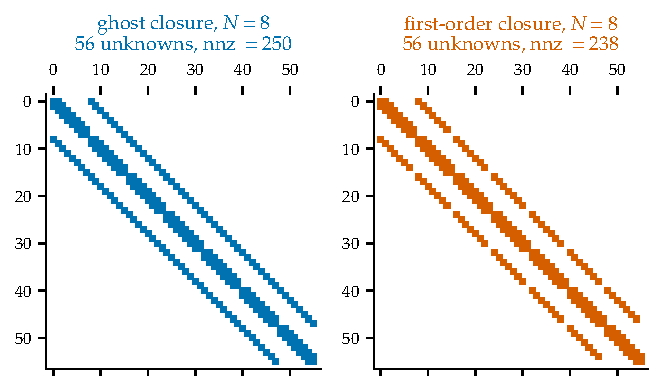
\includegraphics[width=\textwidth]{spy.pdf}\par\vspace{0.4mm}
\figcap{Sparsity of $A$, $N=8$: ghost 250 nnz vs first-order 238; differ only on right-edge rows.}
\figend{}
\end{columns}
\end{frame}

% ============================================================ surface
\begin{frame}{Solution surface: exact, numerical, error}
\bodytop
\centering
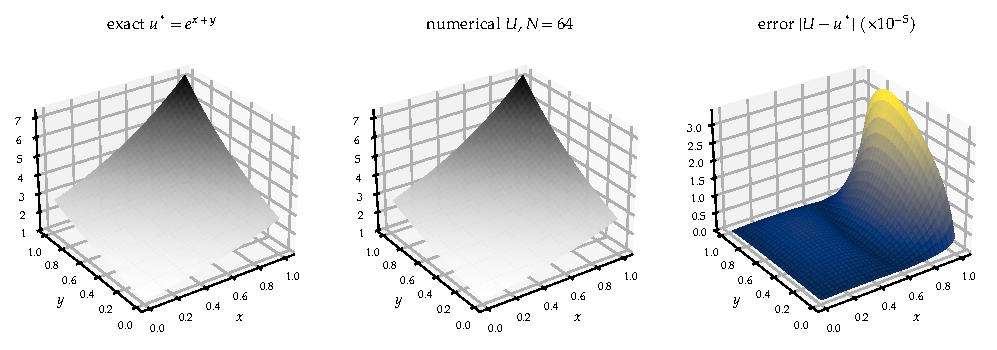
\includegraphics[width=\textwidth,height=50mm,keepaspectratio]{solution_surface.pdf}\par\vspace{2.0mm}
\figcap{Robin ($\beta=2$), ghost closure, $N=64$. $|U-u^*|\le3.34\times10^{-5}$ on $\GB$; vanishes at Dirichlet edges.}
\figend{$U$ matches $u^*=e^{x+y}$; the flux-edge closure sets the accuracy.}
\end{frame}

% ============================================================ 9 convergence
\begin{frame}{Convergence: orders ${\approx}\,1$ and $2$, in both norms}
\bodytop
\centering
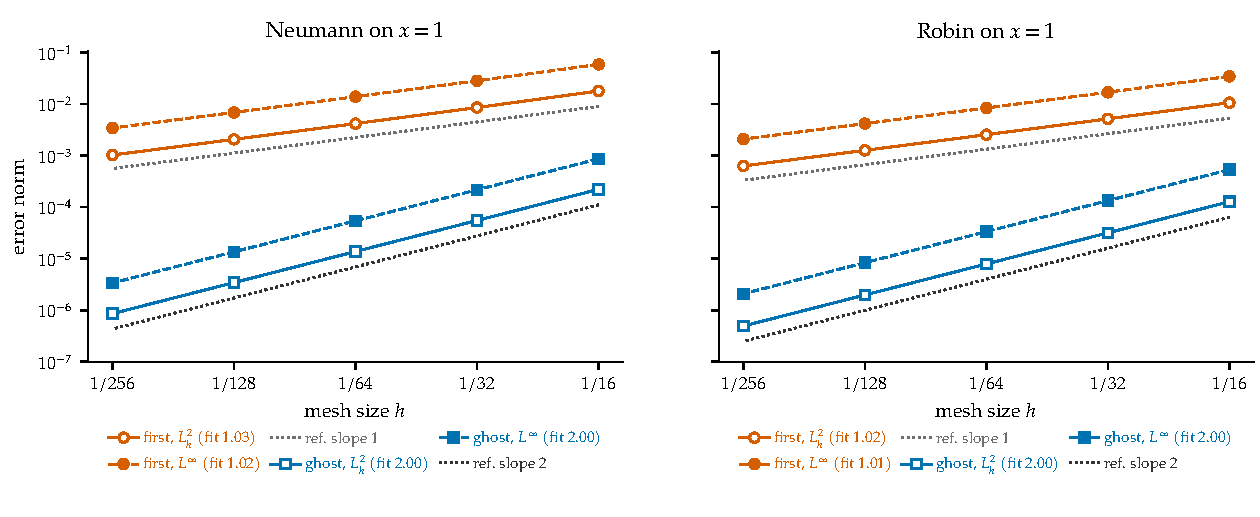
\includegraphics[width=0.96\textwidth,height=51mm,keepaspectratio]{convergence.pdf}\par\vspace{2.4mm}
\figcap{Fit, all levels: $L^2_h$ order 1.03/2.00 (Neu.), 1.02/2.00 (Rob.); max log-dev $\le0.016$.}
\figend{Asymptotic from $N=32$: pairwise $p\in[1.00,1.07]$ and $[1.99,2.01]$. Max error on $\GB$.}
\end{frame}

% ============================================================ 9b errors vs bounds
\begin{frame}{Observed orders and errors versus bounds}
\bodytop
{\tabfont\begin{tabular}{@{}llcc@{}}\toprule
 & closure & $p$, $L^2_h$ & $p$, $L^\infty$\\\midrule
Neumann & first & 1.01 & 1.01\\
 & ghost & 2.00 & 2.00\\
Robin & first & 1.00 & 1.00\\
 & ghost & 2.00 & 2.00\\\bottomrule
\end{tabular}}\blockgap
{\color{note}\notesize Last pair $N=128\to256$.\par}
\blockgap
{\tabfont\begin{tabular}{@{}lcccc@{}}\toprule
$N=256$ & $\|e\|_\infty$ Neumann & bound & $\|e\|_{\infty,\mathrm{int}}$ Neumann & $\|e\|_\infty$ Robin\\\midrule
first-order & $3.411\times10^{-3}$ & $3.69h\approx1.4\times10^{-2}$ & $3.373\times10^{-3}$ & $2.075\times10^{-3}$\\
ghost-point & $3.385\times10^{-6}$ & $1.85h^2\approx2.8\times10^{-5}$ & $3.334\times10^{-6}$ & $2.085\times10^{-6}$\\\bottomrule
\end{tabular}}
\blockgap
\begin{itemize}\setlength{\itemsep}{\blockskip}
\item Observed max errors sit below the comparison-function bounds, with factors $\approx4$ (first-order) and $\approx8$ (ghost).
\item Interior max error is almost as large as the global max: the flux-edge closure limits first-order accuracy.
\end{itemize}
\closing{Bounds from the $A\psi$ comparison on slide~8; orders proved $O(h)$ / $O(h^2)$, observed $1.00$--$1.01$ / $2.00$.}
\end{frame}

% ============================================================ 10 cost
\begin{frame}{Cost versus accuracy: matched target $\|e\|_\infty\le5\times10^{-3}$}
\bodytop
Cost: median \textrm{spsolve} time, five runs (assembly, I/O, CG, plots excluded).
\blockgap
{\tabfont\begin{tabular}{@{}llrrrc@{}}\toprule
BC & Closure & $N_{\min}$ (tested) & unknowns & $\|e\|_\infty$ & spsolve (s)\\\midrule
Neumann & first-order & 256 & 65280 & $3.411\times10^{-3}$ & $2.46\times10^{-1}$\\
Neumann & ghost-point & 16 & 240 & $8.611\times10^{-4}$ & $3.48\times10^{-4}$\\
Robin & first-order & 128 & 16256 & $4.159\times10^{-3}$ & $3.80\times10^{-2}$\\
Robin & ghost-point & 16 & 240 & $5.307\times10^{-4}$ & $3.23\times10^{-4}$\\\bottomrule
\end{tabular}}\blockgap
\begin{itemize}\setlength{\itemsep}{\blockskip}
\item Ghost meets the target at $N=16$ (coarsest tested); first-order needs $N=128$ (Robin) or $N=256$ (Neumann). Solve-time ratio $\sim10^{2}$--$10^{3}$.
\item Dotted line on the next slide: tighter reference $10^{-3}$ (not the table target); first-order Neumann at $N=512$ still $1.70\times10^{-3}$.
\end{itemize}
\closing{$N_{\min}$: smallest tested mesh meeting the target, $N\in\{16,32,64,128,256,512\}$. Source: \textrm{results/cost\_accuracy.csv}.}
\end{frame}

% ============================================================ 10b cost curves
\begin{frame}{Cost curves: $\|e\|_\infty$ versus \textrm{spsolve} time}
\bodytop
\centering
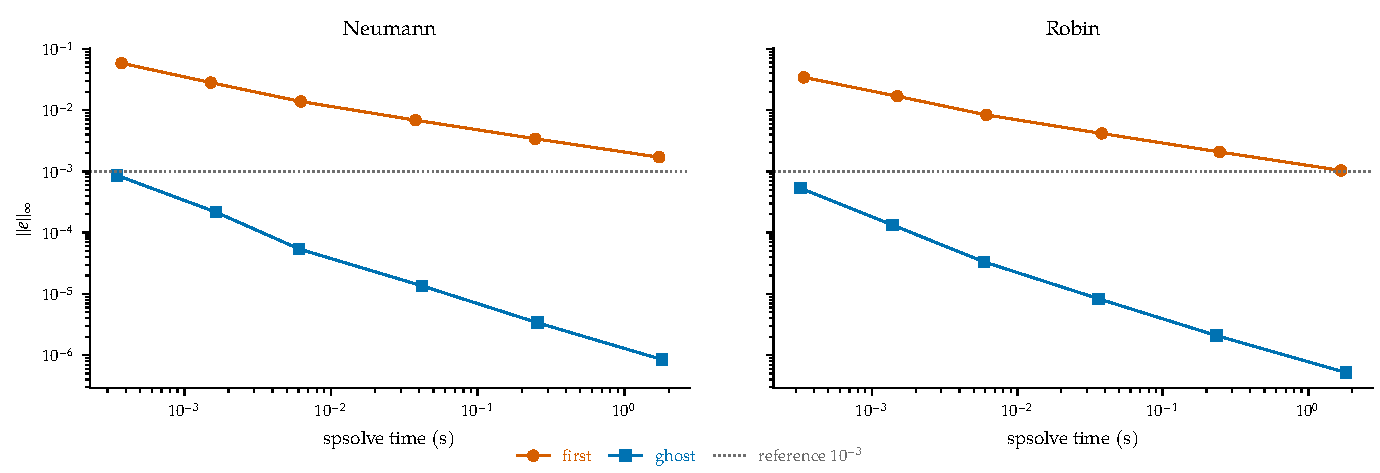
\includegraphics[width=0.96\textwidth,height=51mm,keepaspectratio]{cost_accuracy.pdf}\par\vspace{2.4mm}
\figcap{Dotted line: reference $10^{-3}$ (stricter than the table target $5\times10^{-3}$). Ghost reaches the table target at $N=16$.}
\figend{Same timings as the cost table; assembly, I/O, CG and plots excluded.}
\end{frame}

\section{Close}
% ============================================================ 11 limitations
\begin{frame}{Limitations}
\bodytop
\begin{itemize}\setlength{\itemsep}{\blockskip}
\item One smooth manufactured solution on the unit square. Orders need $C^4$ up to $\GB$; not claimed for nonsmooth or incompatible corner data, or for $\beta<0$.
\item Algebraic vs discretisation error: $\rho\le8.1\times10^{-13}$; CG/direct $\le1.2\times10^{-11}$ at $N=64$; $\kappa_2(DA)\approx2.18\times10^3$ (Robin, ghost, $N=64$), growing like $O(N^2)$.
\item Two check families: MMS substitution, and course analytic bank P1--P5.
\item Cost--accuracy at $\|e\|_\infty\le5\times10^{-3}$ (\textrm{spsolve} only); $10^{-3}$ not reached by first-order within $N\le512$.
\item Package under \textrm{code/} is vectorised.
\item For this manufactured solution, Robin errors are smaller than Neumann at the same mesh resolution.
\end{itemize}
\closing{Optional depth (pure-Neumann nullspace and gauge) not attempted.}
\end{frame}

% ============================================================ 12 conclusion
\begin{frame}{Conclusion and reproducibility}
\bodytop
\begin{itemize}\setlength{\itemsep}{\blockskip}
\item Comparison functions prove $\|e\|_\infty=O(h)$ (first) and $O(h^2)$ (ghost); observed fitted orders ($N=16$--$256$) are $1.01$--$1.03$ and $2.00$ in both norms.
\item The flux-edge closure, not the interior stencil, limits first-order accuracy.
\item Both $A$ are nonsymmetric; diagonal scaling makes $DA$ SPD and legitimises CG.
\item At $\|e\|_\infty\le5\times10^{-3}$ the ghost closure is $10^{2}$--$10^{3}$ times cheaper in \textrm{spsolve} time.
\end{itemize}
\blockgap
\lead{Reproduce.} From \textrm{project2/code/}:
\par\vspace{0.4em}
{\tabfont\begin{tabular}{@{}ll@{}}\toprule
command & produces\\\midrule
\textrm{python run\_all.py} & convergence, MMS checks, cost, figures, tables\\
\textrm{python convergence.py} & \textrm{results/convergence.csv}\\
\textrm{python mms\_runner.py} & truncation, $\kappa$, CG cross-check\\
\textrm{python cost\_accuracy.py} & matched-target timings\\\bottomrule
\end{tabular}}
\closing{Code and data: \href{https://github.com/AXE111111111/321F/tree/main/Project\%202}{\textcolor[RGB]{11,61,145}{\underline{GitHub repository: 321F / Project~2}}}.}
\end{frame}
\end{document}
